%%%%%%%%%%%%%%%%%%%%%%%%%%%%%%%%%%%%%%%%%
% Two Column One Page Curriculum Vitae
% LaTeX Template
% Version 1.1 (24/1/13)
%
% This template has been downloaded from:
% http://www.LaTeXTemplates.com
%
% Original author:
% Alessandro (The CV Inn)
%
% IMPORTANT: THIS TEMPLATE NEEDS TO BE COMPILED WITH XeLaTeX
%
% This template uses several fonts not included with Windows/Linux by
% default. If you get compilation errors saying a font is missing, find the line
% on which the font is used and either change it to a font included with your
% operating system or comment the line out to use the default font.
% 
%%%%%%%%%%%%%%%%%%%%%%%%%%%%%%%%%%%%%%%%%

%----------------------------------------------------------------------------------------
%	PACKAGES AND OTHER DOCUMENT CONFIGURATIONS
%----------------------------------------------------------------------------------------

\documentclass[10pt]{article} % Font size - 10pt, 11pt or 12pt

\usepackage[hmargin=0.25cm, vmargin=1.25cm]{geometry} % Document margins

\usepackage{marvosym} % Required for symbols in the colored box
\usepackage{ifsym} % Required for symbols in the colored box
\usepackage{graphicx}
\graphicspath{ {images/} }
\usepackage[usenames,dvipsnames]{xcolor} % Allows the definition of hex colors

% Fonts and tweaks for XeLaTeX
\usepackage{fontspec,xltxtra,xunicode}
\defaultfontfeatures{Mapping=tex-text}
\setromanfont[Mapping=tex-text]{FreeSans} % Main document font
\setsansfont[Scale=MatchLowercase,Mapping=tex-text]{Purisa} % Font for your name at the top
%\setmonofont[Scale=MatchLowercase]{Andale Mono}

% Colors for links, text and headings
\usepackage{hyperref}
\definecolor{linkcolor}{HTML}{5881ee} % blue color for links
\definecolor{shade}{HTML}{F5DD9D} % Peach color for the contact information box
\definecolor{text1}{HTML}{2b2b2b} % Main document font color, off-black
\definecolor{headings}{HTML}{701112} % Dark red color for headings
% Other color palettes: shade=B9D7D9 and linkcolor=A40000; shade=D4D7FE and linkcolor=FF0080

\hypersetup{colorlinks,breaklinks, urlcolor=linkcolor, linkcolor=linkcolor} % Set up links and colors

\usepackage{fancyhdr}
\pagestyle{fancy}
\fancyhf{}
% Headers and footers can be added with the \lhead{} \rhead{} \lfoot{} \rfoot{} commands
% Example footer:
%\rfoot{\color{headings} {\sffamily Last update: \today}. Typeset with Xe\LaTeX}

%\renewcommand{\headrulewidth}{0pt} % Get rid of the default rule in the header

\usepackage{titlesec} % Allows creating custom \section's

% Format of the section titles
\titleformat{\section}{\color{headings}
\scshape\Large\raggedright}{}{0em}{}[\color{black}\titlerule]

\titlespacing{\section}{0pt}{0pt}{5pt} % Spacing around titles

\begin{document}

\color{text1} % Sets the default text color for the whole document to the color defined as 'text1'

%----------------------------------------------------------------------------------------
%	TITLE
%----------------------------------------------------------------------------------------

%\par{\centering{\sffamily\Huge Ariadni-Karolina Alexiou}\\ % Your name
%{\color{headings}\fontspec[Variant = 2]{FreeSans} Curriculum {Vit\fontspec[Variant = 3]{FreeSans}\ae}\\[15pt]\par} % Curriculum vitae text in the Zapfino font
	
%----------------------------------------------------------------------------------------

\begin{minipage}[t]{0.5\textwidth} % Start the left-hand side of the page
\vspace{0pt} % Trick for alignment
	
%----------------------------------------------------------------------------------------
%	EDUCATION
%----------------------------------------------------------------------------------------



\section{Education} 

\begin{tabular}{rl} % Start a table with two columns, one for dates and one for qualifications



2011 -- 2013 & \textbf{Master of Science} \\ 
& \textsc{Computer Science} \\ 
& \textit{ETH Z\"urich}\\
    \small  & GPA: 5.5/6 (also received scholarship) \\
Master Thesis
& \textbf{Adaptive filters for optimizing range}\\
& \textbf{query processing on data across}\\
& \textbf{multiple physical locations}\\
& \textit{Supervised by Donald Kossmann}\\
	 

2007 -- 2011 & \textbf{Bachelor of Science}\\
& \textsc{Computer Science} \\
& \textit{University of Athens} \\
\small  & GPA: 9.3/10 -- Top graduate in fall 2011\\
	
\end{tabular}\\[9pt]

%----------------------------------------------------------------------------------------
%	WORK EXPERIENCE
%----------------------------------------------------------------------------------------

\section{Work Experience} 

%------------------------------------------------
% WORK EXPERIENCE 1
%------------------------------------------------
{\raggedleft\textsc{September 2017 - Present}\par}

{\raggedright\large \textbf{Fullstack Engineer at siroop, Z\"urich}\\
}

\normalsize{Responsible for web development and development of micro-services using Python. Practising test driven development and agile methodologies. Also managing the AWS infrastructure using Terraform.}
\\
{\raggedleft\textsc{March 2017 - August 2017}\par}

{\raggedright\large \textbf{Data Engineer at siroop, Z\"urich}\\
}

\normalsize{Responsible for data management tasks, maintenance of infrastructure and for developing algorithms for the personalization of a Swiss e-commerce website. Technologies: Amazon Web Services as building blocks for data ingestion and processing, also pyspark, hive and presto. Introduced and set up airflow as a pipeline manager and databricks as a development environment.}
\\
\\
{\raggedleft\textsc{November 2015 - February 2017}\par}

{\raggedright\large \textbf{Lead Data Engineer at Tracktics GmbH, Z\"urich}\\
}

\normalsize{ Responsible for creating internal tools and automated processes to keep the data organized and to evaluate and produce reports for the accuracy of different approaches to fuse GPS with intertial sensor data. Technologies: Python, C and MATLAB.}
\\
\\
{\raggedleft\textsc{September 2013 - June 2015}\par}

{\raggedright\large \textbf{Software Developer at Teralytics AG, Z\"urich}\\
}

\normalsize{Worked with geospatial databases (PostgreSQL), Apache Hadoop, Spark and other data analysis libraries to provide business insights on large volumes of data. Developed solutions for complex data analytics, visualizations, reports, data management and integration in Python, Scala and Java.}
\\
\\
{\raggedleft\textsc{March 2013 - June 2013}\par}

{\raggedright\large \textbf{Software Engineering Intern at Google, Z\"urich}\\
}

\normalsize{Worked with Google Web Toolkit on the Youtube Analytics Team. Responsibilities included database migration and data analysis.}\\


%------------------------------------------------
% WORK EXPERIENCE 2
%------------------------------------------------

%{\raggedleft\textsc{February 2012 -- May 2012}\par}

%{\raggedright\large \textbf{Teaching Assistant for the Data Modeling and Databases course at ETH, Zurich}\\}

%\normalsize{Taught basic and intermediate concepts of databases (eg. UML, Relational Models, Normal Forms, Transactions, SQL operators), created exercises for students and graded their final SQL and Java projects.}\\

%------------------------------------------------
% WORK EXPERIENCE 3
%------------------------------------------------

%{\raggedleft\textsc{March 2011 -- June 2011}\par}

%{\raggedright\large \textbf{Game programmer at 4pi Publications, Athens}\\}

%\normalsize{Created flash games for an educational magazine in ActionScript 3.0, working closely with sound and graphic artists.}\\


%----------------------------------------------------------------------------------------
	

\end{minipage} % End the left-hand side of the page
\hfill
\begin{minipage}[t]{0.44\textwidth} % Start the right-hand side of the page
\vspace{0pt} % Trick for alignment

%----------------------------------------------------------------------------------------
%	COLORED BOX
%----------------------------------------------------------------------------------------

\colorbox{shade}{\textcolor{text1}{
        \begin{tabular}{l|p{5.5cm}}
            \raisebox{-1.25cm}{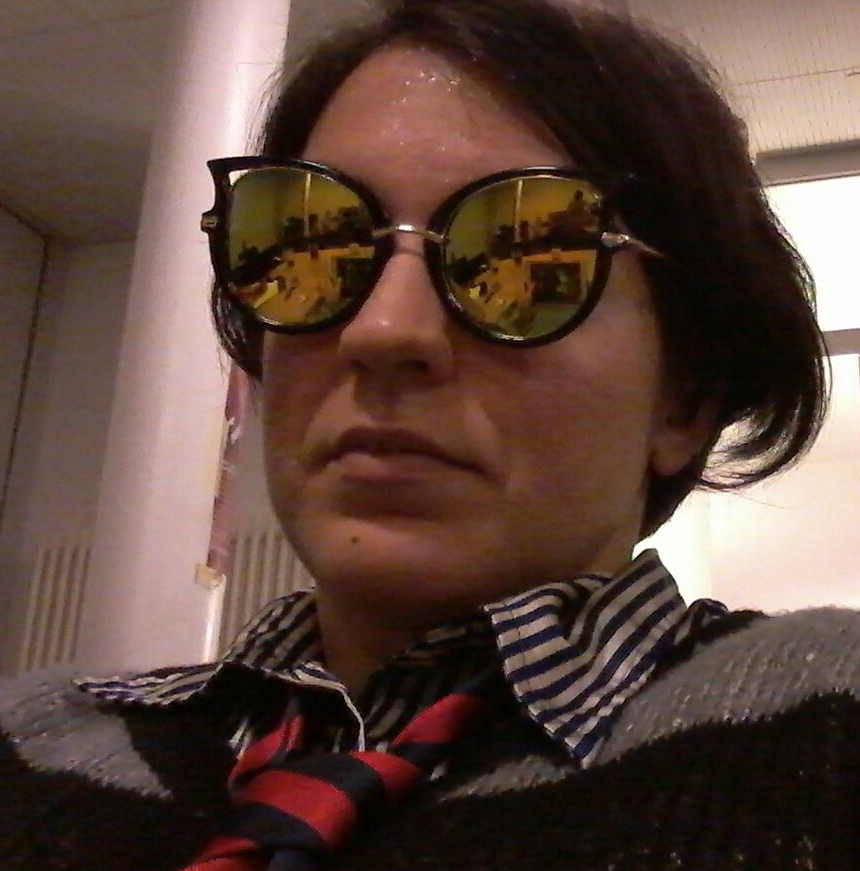
\includegraphics[height=2.5cm]{photo_2018}} &
        \begin{tabular}{l|p{5cm}}
    \raisebox{0pt}{\Smiley} & \textbf{Ariadni-Karolina Alexiou} \\ % Name
    \raisebox{-1pt}{\textifsymbol{18}} & Albisstrasse 35, Z\"urich 8038 \\ % Address
    \raisebox{-1pt}{\Mobilefone} & +41 76 227 1139\\ % Phone number
    \raisebox{-1pt}{\Letter} & carolinegr@gmail.com \\ % Email address
    \Keyboard & \href{http://www.github.com/carolinux}{http://www.github.com/carolinux} \\ % Github
        \end{tabular}  \\ % Name
\end{tabular}
}
}\\[10pt]





%----------------------------------------------------------------------------------------
%	COMPUTER SKILLS
%----------------------------------------------------------------------------------------

\section{Core Competencies} 
    \normalsize{\textbf{Data Science} - Loading, exploring, creating interactive reports/visualizations for data in Python, combining diverse datasets and APIs, applying statistical methods.}\\
    \\
    \normalsize{\textbf{Data Engineering} - Productization of data science prototypes, managing communication between engineers and data scientists, building data pipelines and creating tools for continuous evaluation and data management.}\\
    \\
    \normalsize{\textbf{Big Data} - Experience with PostgreSQL, Hadoop and Scala/Spark, celery to do quicker computations. }\\
    \\
\normalsize{\textbf{Full stack development} with Flask/Django, creating APIs, jQuery (focus on backend). }\\
\\
\normalsize{\textbf{Devops} - Automating deployment of data pipelines and other tools with Ansible. }\\
\\
\normalsize{\textbf{Geospatial Data} - Familiar with PostGIS, QGIS and have co-authored a \href{http://github.com/anitagraser/TimeManager}{plugin for interactive visualization of geotemporal data.}}\\

%Languages
%& \textsc{Python}, \textsc{Java}, \textsc{Scala} \\
%& \textsc{C/C++}, \textsc{VHDL}, \textsc{SQL} \\
%& \textsc{PHP}, \textsc{HTML}, \textsc{bash} \\
%& \textsc{JavaScript}, \textsc{\LaTeX} \\
%&\\
%Frameworks
%& Hadoop, Spark, pandas \\
%& Redis, MongoDB, PostgreSQL \\
%& JQuery, d3 \\
%& Boost, CGAL \\
%& Adobe Flash, FlashDevelop \\
%& MATLAB, R, QGIS \\
%& Open Office, Eclipse, IDEA, Vim\\


%\end{tabular}






%----------------------------------------------------------------------------------------
%	COMMUNICATION SKILLS
%----------------------------------------------------------------------------------------

%2010 (athens)	
%Volunteer in the 6th Hellenic Conference on Artificial Intelligence
%2008 – 09 (athens)	 Participation in Microsoft Imagine Cup
%2008 (samos)	 Panhellenic Conference on Informatics
%2008 (athens)	 3IA International Conference on Computer Graphics

\section{Selected Conferences and Articles} 

\begin{tabular}{rl}
\textsc{2016}
& Published reflections on the future of \href{http://www.datasciencecentral.com/profiles/blogs/interview-with-karolina-alexiou-building-data-pipelines}{Data Pipelines}\\
& and the future of \href{https://blog.propulsionacademy.com/why-python-for-data-science-is-the-future-b556de75c80c#.mdh3ztapq}{Python for Data Science}\\
\textsc{2015}
& Tutorial with Python code snippets:\\
& \href{https://www.airpair.com/python/posts/using-python-and-qgis-for-geospatial-visualization}{Exploring a UFO sightings dataset}\\
\textsc{2015}
& Article: \href{https://www.airpair.com/python/posts/top-mistakes-python-big-data-analytics}{Common mistakes with Python and Big Data}\\
\textsc{2015}
& Presented workshop at \\
& QGIS user \& dev conference \\
\textsc{2014}
& Presented published paper at \\
& VLDB 2014 (Master Thesis) \\
\textsc{2014}
& Speaker at PyData Berlin conference \\
& on Mall Analytics (from prototype to product) \\ 
%\textsc{2014}
%& Speaker at \\
%& Swiss Postgres conference \\
%& \small Rapperswil, Switzerland \\
%\textsc{2014}
%& Speaker at \\
%& Swiss Big Data User Group Meetup \\
%& \small Z\"urich, Switzerland \\


%\textsc{2009}
%& Participated in Microsoft Imagine Cup \\
%&\small  Athens, Greece\\



\end{tabular}\\[10pt]

	
\end{minipage} % End right-hand side of the page

% teh second page!
\begin{minipage}[t]{0.5\textwidth} % Start the left-hand side of the page
\vspace{0pt} % Trick for alignment
	
%----------------------------------------------------------------------------------------
%	EDUCATION
%----------------------------------------------------------------------------------------


\section{Selected Freelance Work} 


{\raggedright\large \textbf{Python and Data Engineering Tutor, online}\\
}

\normalsize{Micro-consulting via \href{http://www.codementor.io/carolinux}{codementor.io}.}
\\

{\raggedright\large \textbf{Mentor at Andela, online}\\
}

\normalsize{Mentored junior programmers in Python, testing and programming patterns to prepare them for working remotely.} 
\\

{\raggedright\large \textbf{Data Consultant for New Incentives, Z\"urich}\\
}

\normalsize{Created a data pipeline in Scala to sync data daily across mobile devices and Google spreadsheets.}\\
\\
{\raggedright\large \textbf{QGIS Plugin Developer for OpenGis.ch, Z\"urich}\\
}

\normalsize{Responsible for developing Python plugins for geospatial data management.}\\

%------------------------------------------------
% WORK EXPERIENCE 2
%------------------------------------------------

%{\raggedleft\textsc{February 2012 -- May 2012}\par}

%{\raggedright\large \textbf{Teaching Assistant for the Data Modeling and Databases course at ETH, Zurich}\\}

%\normalsize{Taught basic and intermediate concepts of databases (eg. UML, Relational Models, Normal Forms, Transactions, SQL operators), created exercises for students and graded their final SQL and Java projects.}\\

%------------------------------------------------
% WORK EXPERIENCE 3
%------------------------------------------------

%{\raggedleft\textsc{March 2011 -- June 2011}\par}

%{\raggedright\large \textbf{Game programmer at 4pi Publications, Athens}\\}

%\normalsize{Created flash games for an educational magazine in ActionScript 3.0, working closely with sound and graphic artists.}\\


%----------------------------------------------------------------------------------------
	

\end{minipage} % End the left-hand side of the page
\hfill
\begin{minipage}[t]{0.44\textwidth} % Start the right-hand side of the page
\vspace{0pt} % Trick for alignment


\section{Languages} 
\normalsize{English, German and Spanish in full professional capacity. Greek as mother tongue, some French.}\\

\section{Personal Interests} 
\normalsize{Painting (have some professional training), Social Science, Travelling}\\
%----------------------------------------------------------------------------------------
	
\end{minipage} % End right-hand side of the page

\end{document}  
